\documentclass[numerate]{cheatsheet}
\usepackage{bm}
\usepackage{textcomp, mathcomp}
\usepackage{empheq}
\usepackage{pbox}
\usepackage{booktabs}
\usepackage{cancel}
\usepackage{amssymb}
\usepackage{amsmath}

\newcommand{\doubleabs}[1]{\left\| #1 \right\|}
\newcommand{\abs}[1]{\left\lvert #1 \right\rvert}


\doctitle{Control Systems 2 Cheatsheet}
\author{Noa Sendlhofer - nsendlhofer@ethz.ch}

\begin{document}
\section{Discrete Time}
	\subsection{Sampling}
    \begin{minipage}{0.49\linewidth}
        \centering \vspace{4pt}
        $T_s$: Sampling Time\\
        \vspace{2pt}
        $\omega_s$: Sampling frequency\\      
    \end{minipage}
    \begin{minipage}{0.49\linewidth}
        \centering
        $$
            \omega_s = \frac{2\pi}{T_s}
        $$
    \end{minipage}
	\subsection{Aliasing}
    \begin{align*}
        y_1[k] &= cos(\omega k T_s), &&k = 0, 1, 2\\
        y_2[k] &= cos((\omega + n\frac{2\pi}{T_s})k T_s), &&n = 0, 1, 2\\
        &= cos(\omega k T_s + \text{\cancel{$n2\pi k$}}) = y_1[k]
    \end{align*}
    \centerline{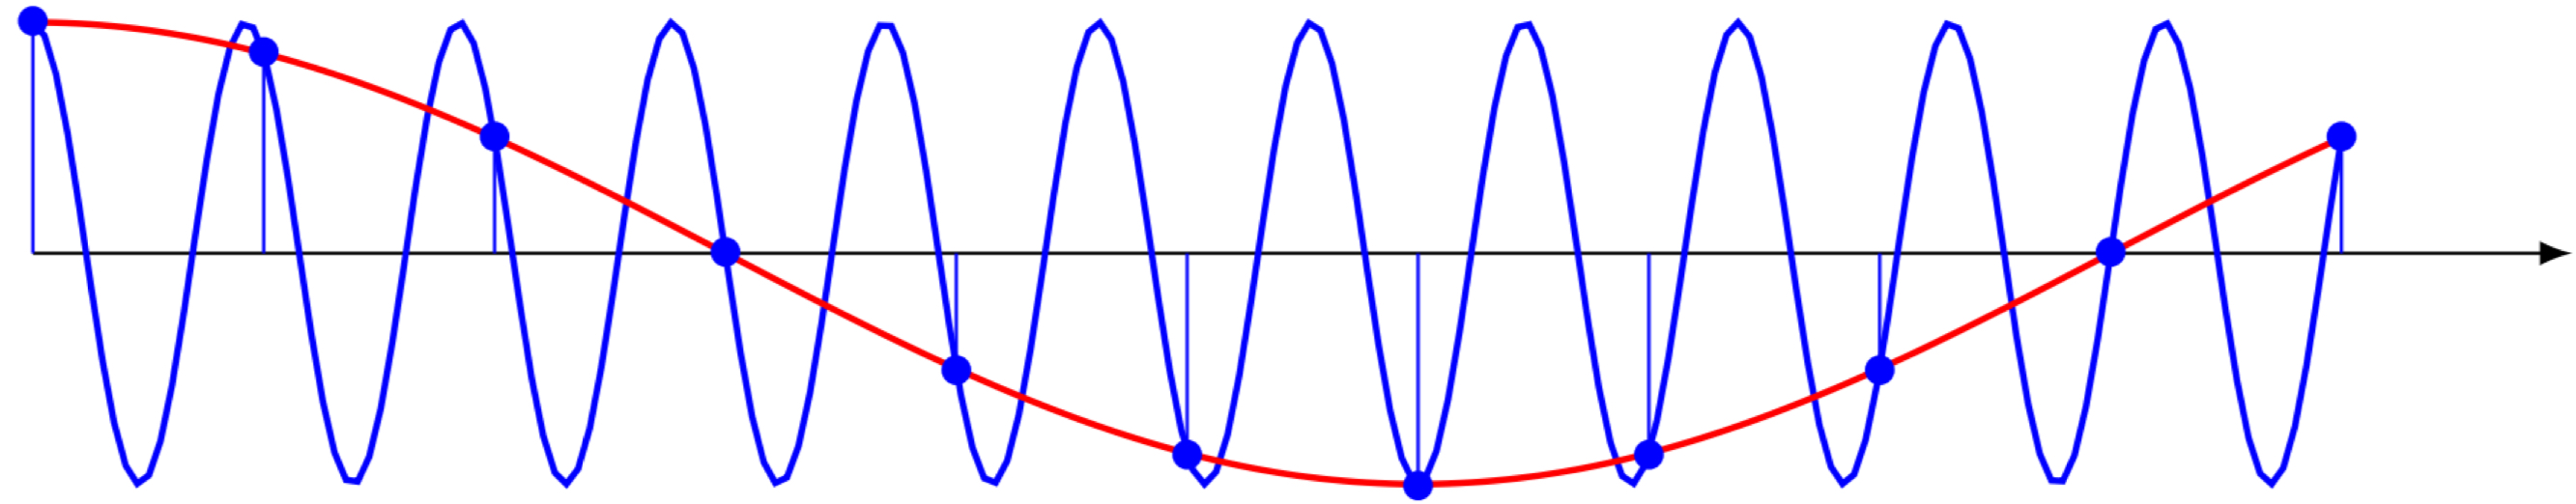
\includegraphics[width=0.8\linewidth]{src/1_discrete_time/images/aliasing.jpg}}
    \vspace{0pt}

    \subsubsection{Nyquist-Shannon Sampling theorem}
        $$
        f_N = \frac{1}{2T_s}\left[\text{Hz}\right] \quad \text{or} \quad \omega_N = \frac{\pi}{T_s}\left[\frac{\text{rad}}{\text{s}}\right]
        $$

        \centerline{\textbf{No aliasing if $\omega < \omega_N$!}}
	\subsection{DT State Space Representation}
    \begin{align*}
        x[k+1] &= A_d x[k] + B_d u[k]\\
        &= e^{A T_s} x[k] + \left(\int_{0}^{T_s} e^{A \tau}d\tau\right)B u[k]\\
        y[k] &= C_d x[k] + D_d u[k]\\
        &= C x[k] + D u[k]
    \end{align*}

    \quad If A is invertible: $B_d = A^{-1}(A_d - I)B$

    \subsubsection{Emulation}
        \centerline{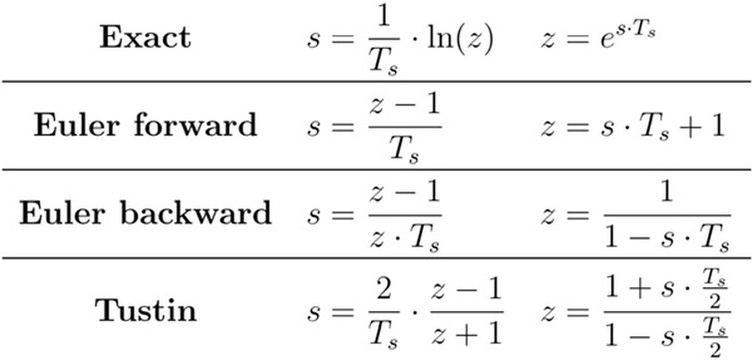
\includegraphics[width=0.8\linewidth]{src/1_discrete_time/images/emulation.jpeg}}
	\subsection{DT Transfer Function}
$$
    u[k] = u_0z^k = u_0e^{ksT} = u(kT)
$$
\begin{align*}
    y[k] &= C\sum_{i=0}^{k-1} A^{k-i-1}Bu_0z^i + Du_0z^k\\
    &= \underbrace{CA^k(x_0-C(zI-A)^{-1}Bu_0)}_{\text{Transient}}\\
    & \; + \underbrace{C(zI-A)^{-1}Bu_0z^k+Du_0z^k}_{\text{Steady-state}}
\end{align*}
$$
    \lim_{k\rightarrow +\infty}A^k = 0 \quad \Rightarrow \quad y[k] \approx [C(zI-A)^{-1}B+D]u[k]
$$
$$
    y[k] \approx G(z)u[k], \quad G(z) := C(zI-A)^{-1}B+D
$$
	\subsection{Approximation Methods}
    \subsubsection{Emulation}
        \centerline{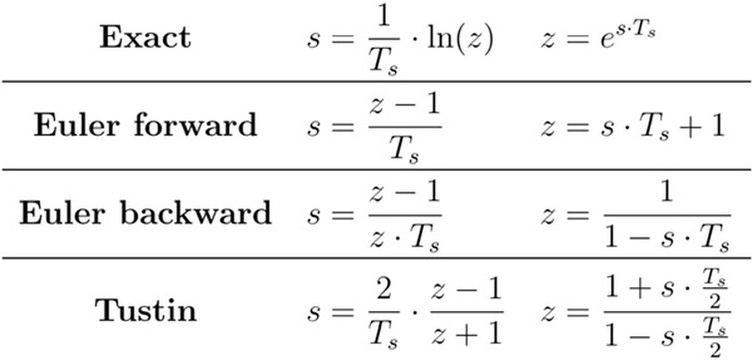
\includegraphics[width=0.8\linewidth]{src/1_discrete_time/images/emulation.jpeg}}
\section{System Properties}
	\subsection{Similarity Transformation}
    \begin{minipage}{0.43\linewidth}
        \vspace{1pt}
        \begin{equation*}
            \left\{
                \begin{aligned}
                    x^+ &= Ax + Bu\\
                    y &= Cx + Du
                \end{aligned}
            \right. \parbox[t]{0.7cm}{$\quad\Longrightarrow$}
        \end{equation*} 
    \end{minipage}
    \begin{minipage}{0.56\linewidth}
        \begin{equation*}
            \left\{
                \begin{aligned}
                    \tilde{x}^+ &= (T^{-1}AT)\tilde{x} + (T^{-1}B)u\\
                    y &= (CT)\tilde{x} + Du
                \end{aligned}
            \right.
        \end{equation*}
    \end{minipage}
    \vspace{2pt}

\subsubsection{Modal decomposition}
\vspace{-5pt}
\begin{minipage}{0.49\linewidth}
    \begin{equation*}
        \tilde{x}_i(t) = e^{\lambda_it}\tilde{x}_i(0)
    \end{equation*} 
\end{minipage}
\begin{minipage}{0.49\linewidth}
    \begin{equation*}
        x(t) = \sum_{i=1}^{n}e^{\lambda_it}\tilde{x}_i(0)v_i
    \end{equation*}
\end{minipage}
\vspace*{0.2em}
	\subsection{Reachability}
    \begin{minipage}{0.63\linewidth}
        $$
        \mathcal{R} := \left[A^{n-1}B | ... | AB | B \right] \in \mathbb{R}^{n\times n \cdot m}
        $$
    \end{minipage}
    \begin{minipage}{0.36\linewidth}
        $$
            U :=
            \begin{bmatrix}
                u[0] \\
                u[1] \\
                \vdots \\
                u[n -1]
            \end{bmatrix}
        $$
    \end{minipage}

    $\Rightarrow x[n] = \mathcal{R}U$
    \vspace{5pt}

    \textbf{The systen is reachable if and only if $\mathcal{R}$ has full row rank n}
	\subsection{Observability}
    \begin{minipage}{0.33\linewidth}
        \centering
        $\mathcal{O} = \begin{bmatrix} \strut C \\ \strut CA \\ \raisebox{0.5ex}{\vdots} \\  \strut CA^{n-1} \end{bmatrix}$
    \end{minipage}
    \begin{minipage}{0.32\linewidth}
        \centering
        $Y = \begin{bmatrix} \strut y[0] \\ \strut y[1] \\ \raisebox{0.5ex}{\vdots} \\ \strut y[n-1] \end{bmatrix}$
    \end{minipage}
    \begin{minipage}{0.32\linewidth}
        \centering
        $Y = \mathcal{O}x[0]$
    \end{minipage}
    \vspace{3pt}

    \textbf{The systen is observable if and only if $\mathcal{O}$ has full column rank n}
	\subsection{Controllability}
    A system is controllable if, for any initial condition $x_0$, there exists a control input $u$ that brings the state $x$ to $0$ in finite time.

    For CT Systems: Controllability = Reachability

    For DT Systems: A is invertible $\Rightarrow$ Controllability = Reachability
	\subsection{Kalman Decomposition}
\begin{align*}
    x^+ &= \begin{bmatrix}
        \Lambda_{r\overline{o}} & 0 & 0 & 0 \\
        0 & \Lambda_{ro} & 0 & 0 \\
        0 & 0 & \Lambda_{\overline{r}\overline{o}} & 0 \\
        0 & 0 & 0 & \Lambda_{\overline{r}o}
    \end{bmatrix} x + 
    \begin{bmatrix}
        B_{r\overline{o}} \\
        B_{ro} \\
        0 \\
        0
    \end{bmatrix} u, \\
    y &= \begin{bmatrix}
        0 & C_{ro} & 0 & C_{\overline{r}o}
    \end{bmatrix} x + Du
\end{align*}

\begin{itemize}
    \item \textbf{Stabilizability}\\
        A system is said to be stabilizable if all unstable modes are reachable

    \item \textbf{Detectability}\\
        A system is said to be detectable if all unstable modes are observable
\end{itemize}
\section{State Feedback}
	\subsection{State Feedback}
\centerline{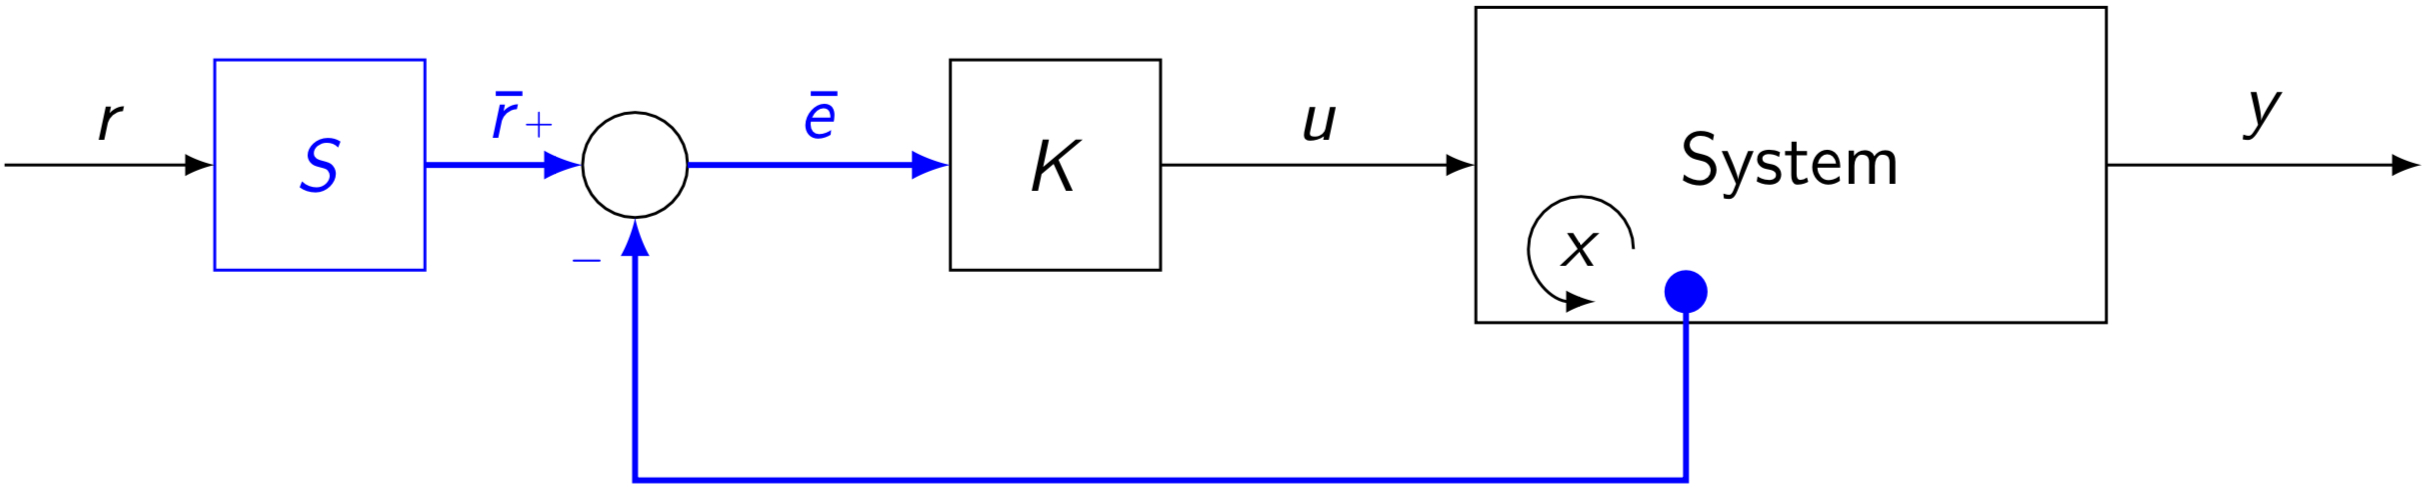
\includegraphics[width=0.95\linewidth]{src/3_state_feedback/images/state_feedback.jpeg}}
\begin{align*}
    \dot{x} &= (A-BK)x + BKSr\\
    &= (A-BK)x + B\overline{N}r, \qquad \overline{N} = KS\\
    y &= Cx + (D=0)\\[5pt]
    G_{yr}^{cl}(s) &= C(sI - A + BK)^{-1}BKS\\
    &= C(sI - A - BK)^{-1}B\overline{N}
\end{align*}

\subsubsection{$K$ - Direct Method}
$$
    p_{cl}^* = \prod_{i=1}^{n}(s + \lambda_i), \quad K = \begin{bmatrix} k_1 & k_2 & \hdots & k_n \end{bmatrix}
$$
$$
    p_{cl} = det(sI - A + BK) = p_{cl}^*
$$

\subsubsection{$K$ - Ackermann's Formula}
$$
    K = \begin{bmatrix} 0 & \hdots & 0 & 1 \end{bmatrix} \mathcal{R}^{-1}p_{cl}^*(A)
$$
\vspace*{0.1em}

\subsubsection{$S$}
$$
    \text{No steady-state error:} \Rightarrow G_{yr}^{cl}(0) = 1
$$
$$
    \Longrightarrow \overline{N} = - (C(A-BK)^{-1}B)^{-1}, \quad S = K^{-1}\overline{N}
$$
\vspace*{0.1em}
	\subsection{LQR}
LQR guarantees:
\begin{itemize}
    \item phase margin $\geq 60^\circ$
    \item gain margin ($\frac{1}{2}, +\infty$)
\end{itemize}

\subsubsection{Continuous Time}
    \vspace*{-0.4em}
    \begin{align*}
        \underset{K}{\text{min}} \, J(x,u) &= \int_{0}^{+\infty}[x(t)^TQx(t) + u(t)^TRu(t)]dt,\\[5pt]
        \text{s.t.:} \quad \dot{x}(t) &= Ax(t) + Bu(t),\\
        u(t) &= -Kx(t)\\[5pt]
        \text{soln.:} \qquad 0 &= A^TX + XA + Q - XBR^{-1}B^TX\\
        K &= R^{-1}B^TX
    \end{align*}

\subsubsection{Discrete Time}
    \vspace*{-0.4em}
    \begin{align*}
        \underset{K}{\text{min}} \, J(x,u) &= \sum_{k=0}^{+\infty}(x[k]^TQx[k] + u[k]^TRu[k]),\\[5pt]
        \text{s.t.:} \quad x[k+1] &= Ax[k] + Bu[k],\\
        u[k] &= -Kx[k]\\[5pt]
        \text{soln.:} \qquad X &= A^TXA - (A^TXB)(B'XB+R)^{-1}(B^TXA)\\
        &+Q\\
        K &= (R+B^TXB)^{-1}B^TXA
    \end{align*}

\subsubsection{LQR Servo}
    $$
    \begin{bmatrix} x \\ \epsilon \end{bmatrix} ^+
    = \begin{bmatrix} A & 0 \\ -C & 0 \end{bmatrix} \begin{bmatrix} x \\ \epsilon \end{bmatrix}
    + \begin{bmatrix} B \\ 0 \end{bmatrix} u + \begin{bmatrix} 0 \\ I \end{bmatrix} r
    $$
\section{State Estimation}
	\subsection{Luenberger Observer}
    \centerline{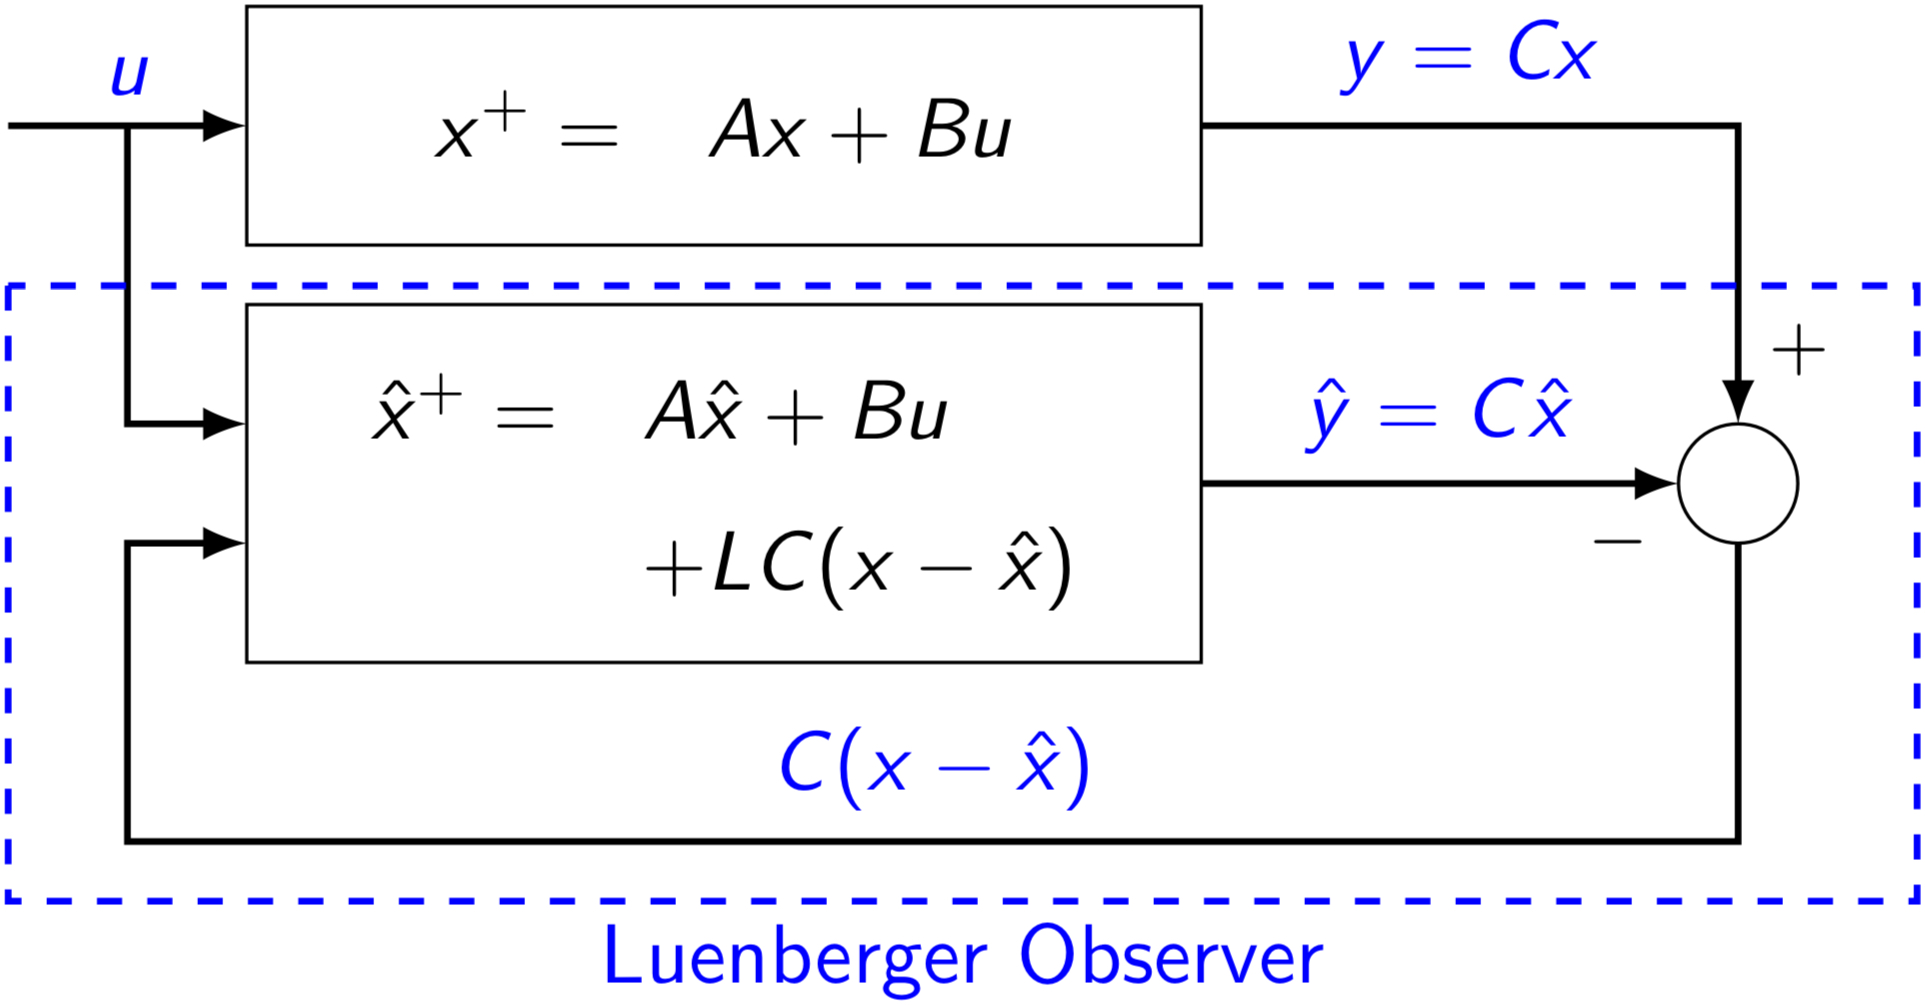
\includegraphics[width=0.8\linewidth]{src/4_state_estimation/images/luenberger_observer.jpeg}}
    \vspace*{-1em}
    \begin{align*}
        \dot{\hat{x}}(t) &= (A-LC)\hat{x}(t) + Bu(t) + Ly(t)\\
        \hat{y}(t) &= C\hat{x}(t)
    \end{align*}
    $$
    \Rightarrow \textbf{Exactely the same as finding a control gain $K$}
    $$
    $$
    L = p_{cl}^*(A)\mathcal{O}^-1[0, \hdots, 0, 1]^T
    $$
	\subsection{LQE}
$$
    Q = \mathbb{E}[w(t)w(t)^T], \quad R = \mathbb{E}[n(t)n(t^T)], \quad \forall t\geq 0
$$
Problem: Find L, such that the steady-state covariance of the state error is minimized.

\textbf{Solution:}
\begin{align*}
    0 &= AY + YA^T - YC^TR^{-1}CY + Q\\
    L &= -YC^TR^{-1}
\end{align*}
\section{Dynamic Output Feedback}
	\centerline{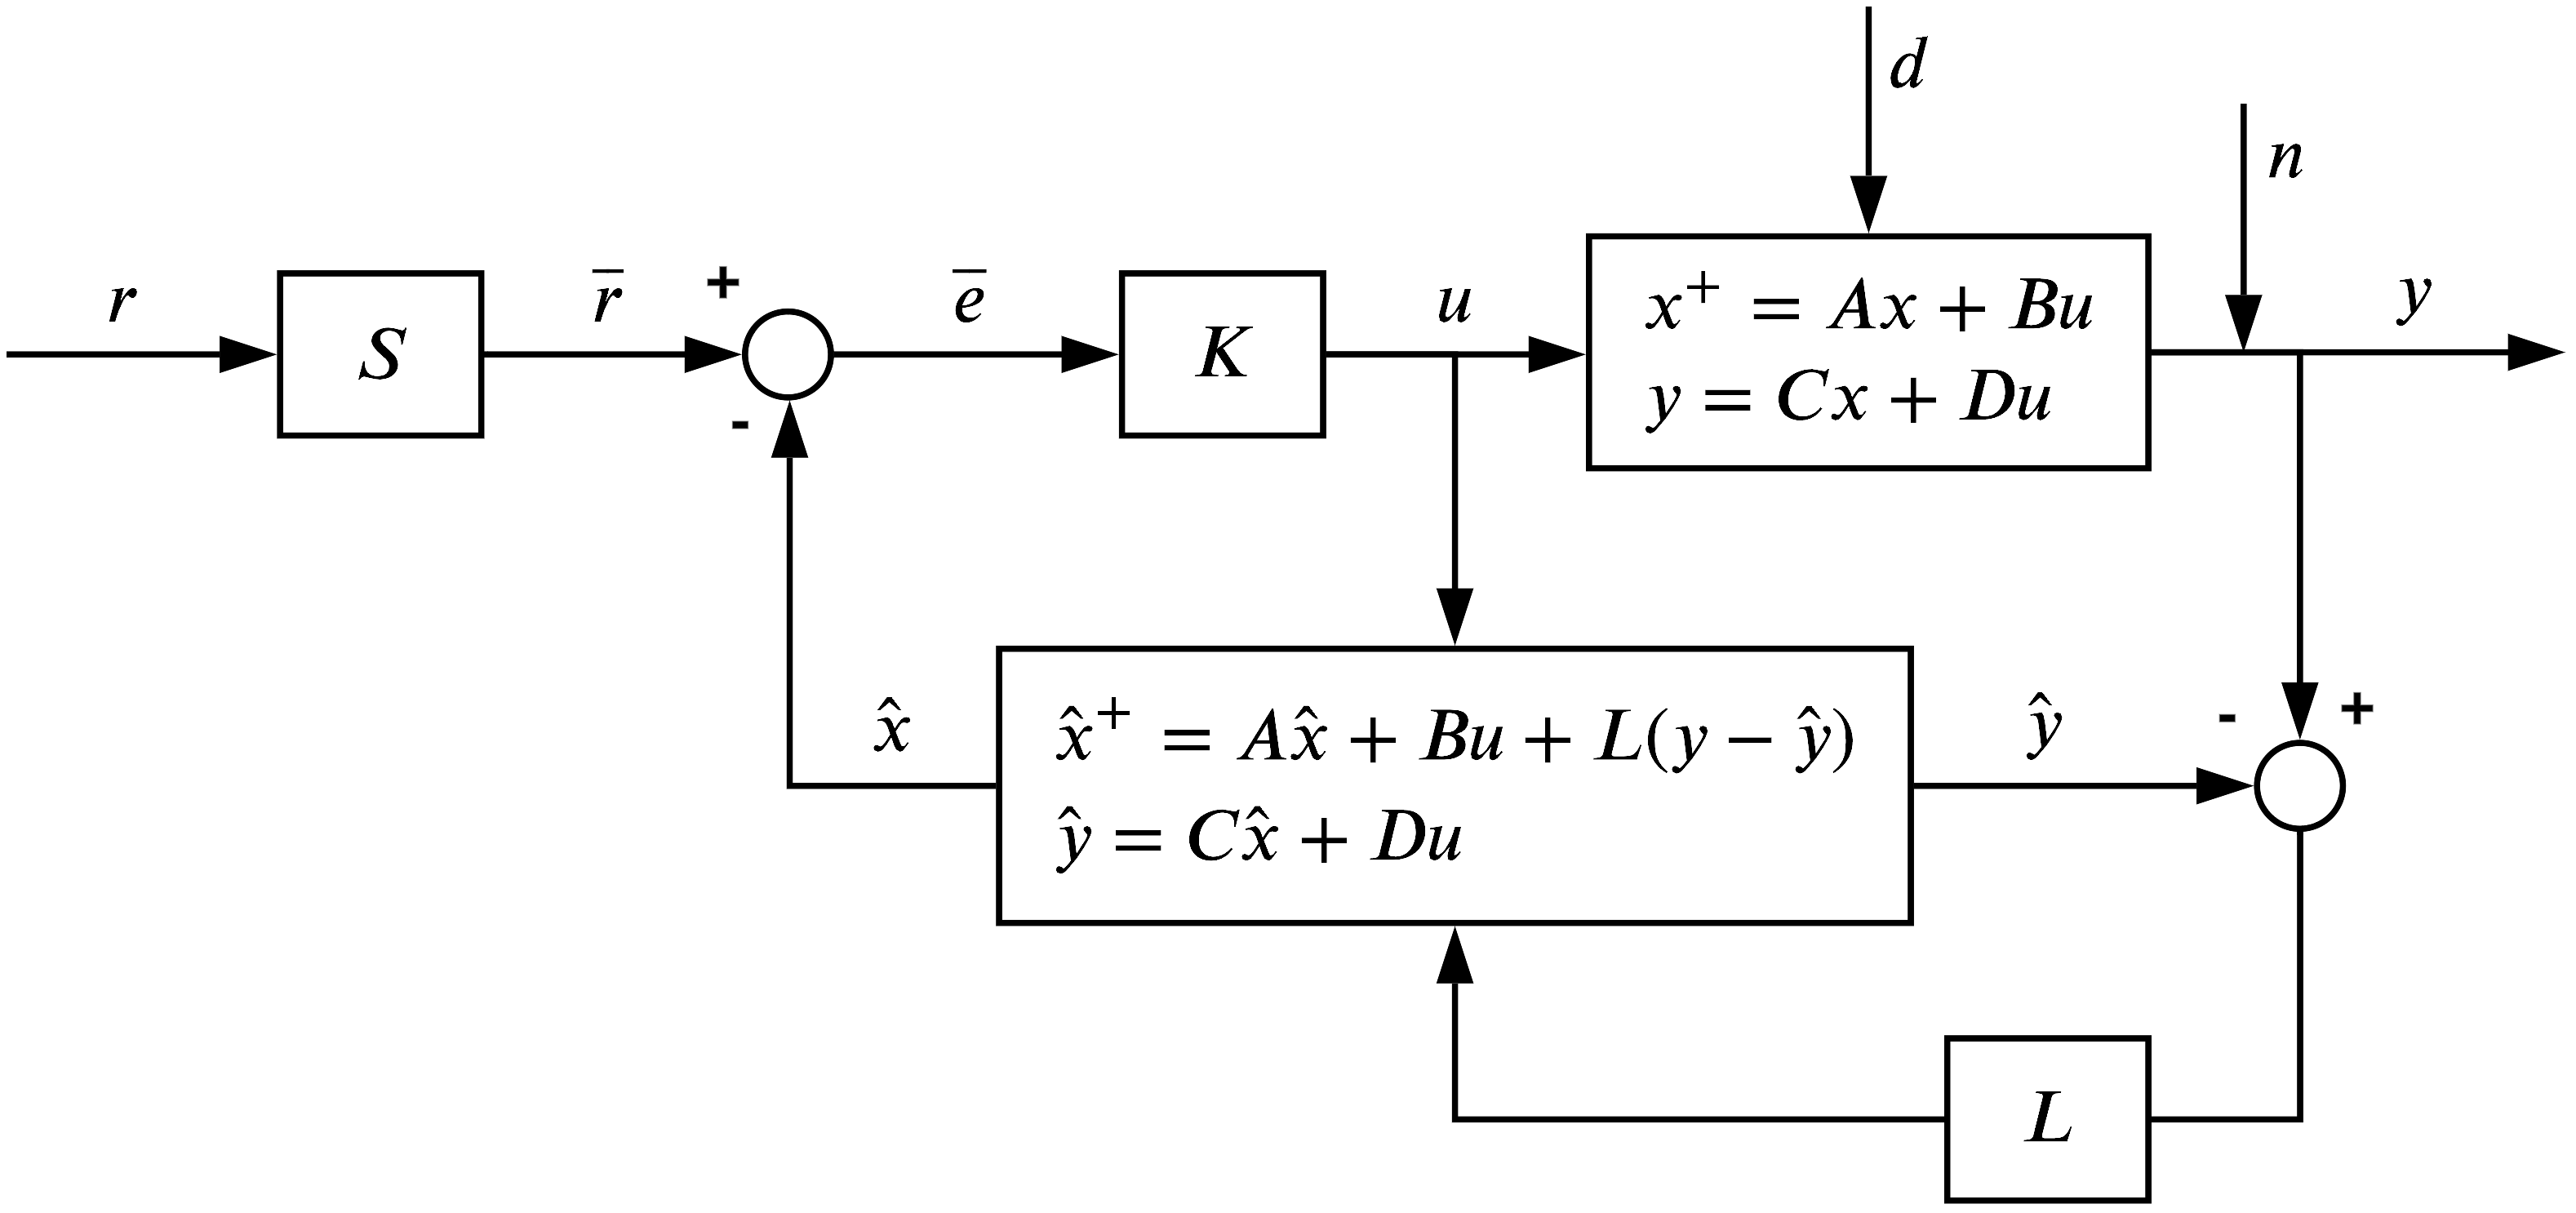
\includegraphics[width=1\linewidth]{src/5_dynamic_output_feedback/images/dofb.png}}

\subsection{LQG}
\begin{align*}
    \begin{bmatrix}
        x \\
        \eta
    \end{bmatrix}^+
    &= \begin{bmatrix}
        A - BK & BK \\
        0 & A - LC
    \end{bmatrix}
    \begin{bmatrix}
        x \\
        \eta
    \end{bmatrix} +
    \begin{bmatrix}
        BKS\\
        0
    \end{bmatrix} r\\
    y &= \begin{bmatrix} C & 0 \end{bmatrix}
    \begin{bmatrix}
        x \\
        \eta
    \end{bmatrix}
\end{align*}

\subsubsection{LQG Servo}
\begin{align*}
    \begin{bmatrix}
        x \\
        x_I \\
        \eta
    \end{bmatrix}^+\!
    &=\! \begin{bmatrix}
        A - BK & -BK_I & BK \\
        -C & 0 & 0 \\
        0 & 0 & A - LC
    \end{bmatrix}\!
    \begin{bmatrix}
        x \\
        x_I \\
        \eta
    \end{bmatrix}\! + \!
    \begin{bmatrix}
        BKS \\
        I \\
        0
    \end{bmatrix}\! r\\
    y &= \begin{bmatrix} C & 0 & 0 \end{bmatrix}
    \begin{bmatrix}
        x \\
        x_I \\
        \eta
    \end{bmatrix}
\end{align*}

\subsubsection{LQG Stability}
LQG guarantees closed loop stability, but the margins can be arbitrarily small.
\section{MIMO}
	\subsection{Transfer Function}
\centerline{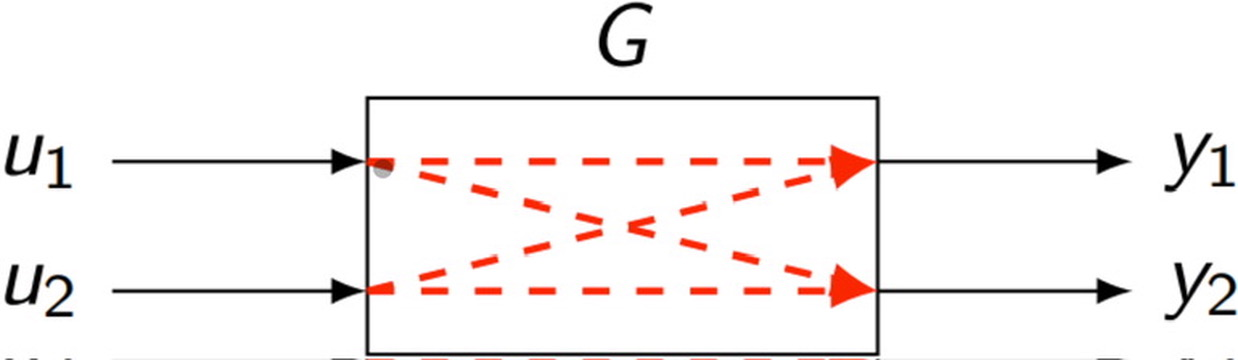
\includegraphics[width=0.5\linewidth]{src/6_mimo/images/transfer_function.jpeg}}

\begin{minipage}{0.55\linewidth}
    \vspace{1pt}
    \begin{equation*}
        \begin{pmatrix}
            y_1 \\
            y_2
        \end{pmatrix} =
        \begin{pmatrix}
            G_{11} & G_{12} \\
            G_{21} & G_{22}
        \end{pmatrix}
        \begin{pmatrix}
            u_1 \\
            u_2
        \end{pmatrix}
    \end{equation*} 
\end{minipage}
\begin{minipage}{0.44\linewidth}
    \begin{equation*}
        G(s) = \begin{pmatrix}
            G_{11} & G_{12} \\
            G_{21} & G_{22}
        \end{pmatrix}
    \end{equation*}
\end{minipage}
\vspace*{0.5em}

\textbf{Push through identity}
\vspace*{-0.5em}
$$
    G_1(I + G_2 G_1)^{-1} = (I + G_1 G_2)^{-1} G_1
$$

\textbf{MIMO state space to tf}
\vspace*{-0.5em}
$$
    G(s) = C(sI - A)^{-1}B + D
$$
	\subsection{State Space}
\begin{align*}
    x^+ &= \underbrace{A}_{n \times n} \underbrace{x}_{n \times 1} + \underbrace{B}_{n \times m} \underbrace{u}_{m \times 1}\\
    y &= \underbrace{C}_{l \times n} \underbrace{x}_{n \times 1} + \underbrace{D}_{l \times m} \underbrace{u}_{m \times 1}
\end{align*}
\begin{itemize}
    \item $x \in \mathbb{R}^n$, where $n$ is the order of the system
    \item $u \in \mathbb{R}^m$, where $m$ is the number of inputs
    \item $y \in \mathbb{R}^l$, where $l$ is the number of outputs
\end{itemize}
	\subsection{MIMO Poles}
MIMO poles are the roots of the pole polynomial of a minimal realization of the transfer function matrix. It is equal to the least common multiple of the denominators of all possible minors of the transfer function.
	\subsection{MIMO Zeros}
\subsubsection{Transmission Zeros}
    $H(s)$ has a transmission zero at frequency $\zeta_0$ if $H(s)$ drops rank at $s = \zeta_0$. In this case the null space of the matrix is non-zero, which means a zero has to exist. $\textrm{rank}(A)+\textrm{nullity}(A)=n$
    \begin{align*}
        H(s) &= \begin{bmatrix}
                    1 & \frac{1}{s-3} \\
                    0 & 1
                \end{bmatrix}\\
        \lim_{s\rightarrow 3} \begin{bmatrix}
                                1 & \frac{1}{s-3} \\
                                0 & 1
                              \end{bmatrix}
        &\Rightarrow \begin{bmatrix}
                        1 & \infty \\
                        0 & 1
                    \end{bmatrix}
        \approx \begin{bmatrix}
                    1 & \infty \\
                    0 & 0
                \end{bmatrix}
    \end{align*}
    \quad $\Longrightarrow \zeta_0$ is a pole and a zero!
    $$
    \lim_{s\rightarrow \zeta_0} H(s)u_0(s) = 0, \quad u_0(s) \; \text{is called "direction"}
    $$

\subsubsection{Invariant Zeros}
    A non-zero input frequency, that doesn't show up in the output. The output can still be non-zero. The invariant zeros correspont to the values $s_i$ for which the matrix
    $$
    \begin{bmatrix}
        sI-A & -B \\
        C & D
    \end{bmatrix}
    $$
    becomes singular. (not full rank)\\
    If the system realization is minimal: invariant zeros $\hat{=}$ transmission zeros.
	\subsection{Gilbert's realization}
\section{Norms}
	\subsection{Definitions}
    \begin{itemize}
        \item $U \in \mathbb{R}^{n \times n}$ is \textbf{orthogonal} if $U^TU = I$
        \item $U \in \mathbb{C}^{n \times n}$ is \textbf{unitary} if $U'U = I$\\ ($U' :=$ complex conjugate transpose)
        \item S is \textbf{hermitian} if $S=S'$\\ For any hermitian $S$, there exists a unitary matrix $U$ s.t. $U'SU$ is diagonal.
    \end{itemize}
    \vspace*{-1em}
    \begin{align*}
        \doubleabs{x}_p &= \left(\sum_{i=1}^{n}x_i^p\right)^{\frac{1}{p}}\\
        \doubleabs{x}_\infty &= \max_{1\leq i\leq n} \left\lvert x_i \right\rvert\\
        \doubleabs{A}_{p,\text{ind}} &= \sup_{x \neq 0} \frac{\doubleabs{Ax}_p}{\doubleabs{x}_p} = \max_{\doubleabs{x}_p = 1} \doubleabs{Ax}_p\\
        \doubleabs{A}_F &= \left( \textrm{Trace}(A'A) \right)^{\frac{1}{p}}
    \end{align*}
	\subsection{Singular Value Decomposition}   
\begin{minipage}{0.2\linewidth}
    \begin{equation*}
        A = U\Sigma V'
    \end{equation*} 
\end{minipage}
\begin{minipage}{0.3\linewidth}
    \begin{equation*}
        \left\{
            \begin{aligned}
                U &\in \mathbb{C}^{m \times m}\\
                V &\in \mathbb{C}^{n \times n}\\
                \Sigma &\in \mathbb{R}^{m \times n}\\
            \end{aligned}
        \right.
    \end{equation*}
\end{minipage}
\begin{minipage}{0.49\linewidth}
    \begin{itemize}
        \item $U,V$ are unitary matrices
        \item $\Sigma$ is diagonal with non-zero entries
    \end{itemize}
\end{minipage}
$$
A = \overbrace{\begin{pmatrix} \underline{u}_1 & \underline{u}_2 \end{pmatrix}}^U
\overbrace{\begin{pmatrix}
    \sigma_1 & 0 \\
    0 & \sigma_2
\end{pmatrix}}^\Sigma
\overbrace{\begin{pmatrix} \underline{v}_1 & \underline{v}_2 \end{pmatrix}'}^{V'}
$$
\begin{itemize}
    \item $u_i$ are the left singular vectors ($\textbf{normalized} \; eig(AA')$)
    \item $v_i$ are the right singular vectors ($\textbf{normalized} \; eig(A'A)$)
    \item $\sigma_i = \sqrt{\lambda_i}$ 
    \item $v_i$ is the specific input that generates the extremal output $u_i$ with amplification $\sigma_i$
\end{itemize}
$$
    \doubleabs{A}_{2,\text{ind}} = \sup_{x \neq 0} \frac{\doubleabs{Ax}_2}{\doubleabs{x}_2} = \sigma_{\textrm{max}}(A)
    , \; \inf_{x \neq 0} \frac{\doubleabs{Ax}_2}{\doubleabs{x}_2} = \sigma_{\textrm{min}}(A)
$$
	\subsection{Signal Norms}
\vspace*{-1em}
\begin{align*}
    \doubleabs{u}_{\mathcal{L}_p} &= \left(\int_{0}^{\infty} \abs{u(t)}^p dt \right)^{\frac{1}{p}}, \quad p \geq 1\\
    \doubleabs{u}_{\mathcal{L}_\infty} &= \sup_{t} \abs{u(t)}\\
    \doubleabs{G}_{\mathcal{H}_2} &= \left(\frac{1}{2\pi}\int_{-\infty}^{\infty} \abs{G(j\omega)}^2 d\omega \right)^{\frac{1}{2}}\\
    \doubleabs{G}_{\mathcal{H}_\infty} &= \sup_{u \neq 0} \frac{\doubleabs{y}_{\mathcal{L}_2}}{\doubleabs{u}_{\mathcal{L}_2}} 
    = \sup_{\omega \in \mathbb{R}} \sigma_{\max}[G(j\omega)]\\
    \doubleabs{u(t)}^2_{\mathcal{L}_2} &= \int_{0}^{\infty} \doubleabs{u(t)}^2_2 dt = \frac{1}{2\pi} \int_{-\infty}^{\infty} \doubleabs{U(s)}^2_2 d\omega\\
    &= \doubleabs{U(s)}^2_{\mathcal{H}_2}
\end{align*}
\end{document}